\documentclass[11pt]{article}

\usepackage{amsmath, amssymb, amsthm}
\usepackage{tikz}

\theoremstyle{plain}
\newtheorem{thm}{Theorem}[section]
\newtheorem*{thm*}{Theorem}
\newtheorem{prop}[thm]{Proposition}
\newtheorem{lem}[thm]{Lemma}
\newtheorem*{lem*}{Lemma}
\newtheorem{dfn}[thm]{Definition}
\newtheorem{cor}[thm]{Corollary}
\newtheorem{claim}[thm]{Claim}
\newtheorem{conj}[thm]{Conjecture}
\newtheorem{ques}[thm]{Question}
\newtheorem*{rem}{Remark}


\oddsidemargin  0pt
\evensidemargin 0pt
\marginparwidth 40pt
\marginparsep 10pt
\topmargin 0pt
\headsep 10pt
\textheight 8.2in
\textwidth 6.4in
\renewcommand{\baselinestretch}{1.1}

\newcommand{\codeg}{\text{codeg}}
\newcommand{\BBE}{\mathbb{E}}
\newcommand{\BFP}{\mathbf{P}}
\usepackage{amsmath}
\usepackage{amsthm}
\usepackage{amssymb}
\usepackage{mathtools}
\usepackage{hyperref}
\usepackage{url}





\usepackage{graphicx}
\usepackage{caption}
\usepackage{subcaption}

\def\eQb#1\eQe{\begin{eqnarray*}#1\end{eqnarray*}}
\def\eQnb#1\eQne{\begin{eqnarray}#1\end{eqnarray}}
\providecommand{\e}[1]{\ensuremath{\times 10^{#1}}}
\providecommand{\pb}[0]{\pagebreak}
\DeclarePairedDelimiter\ceil{\lceil}{\rceil}
\DeclarePairedDelimiter\floor{\lfloor}{\rfloor}

\newcommand{\E}{\mathrm{E}}
\newcommand{\Var}{\mathrm{Var}}
\newcommand{\Cov}{\mathrm{Cov}}

\def\Qb#1\Qe{\begin{question}#1\end{question}}
\def\Sb#1\Se{\begin{solution}#1\end{solution}}


\newtheoremstyle{quest}{\topsep}{\topsep}{}{}{\bfseries}{}{ }{\thmname{#1}\thmnote{ #3}.}
\theoremstyle{quest}
\newtheorem*{definition}{Definition}
\newtheorem*{theorem}{Theorem}
\newtheorem*{lemma}{Lemma}
\newtheorem*{question}{Question}
\newtheorem*{preposition}{Preposition}
\newtheorem*{exercise}{Exercise}
\newtheorem*{challengeproblem}{Challenge Problem}
\newtheorem*{solution}{Solution}
\newtheorem*{remark}{Remark}
\usepackage{verbatimbox}
\usepackage{listings}
\usepackage{mathrsfs}
\date{}
\title{\vspace{-0.7cm}
Diff Geo II: Problem Set I}

\author{
Youngduck Choi 
\thanks{Department of Mathematics, Courant Institute of Mathematical Sciences, 
yc1104@nyu.edu; If you find an error and want to share with me, 
you can reach me via email.
}}

\begin{document}

\maketitle

\begin{abstract}
This work contains solutions for the problem set I.
\end{abstract}


\begin{question}[1-1]
\hfill
\begin{figure}[h!]
  \centering
    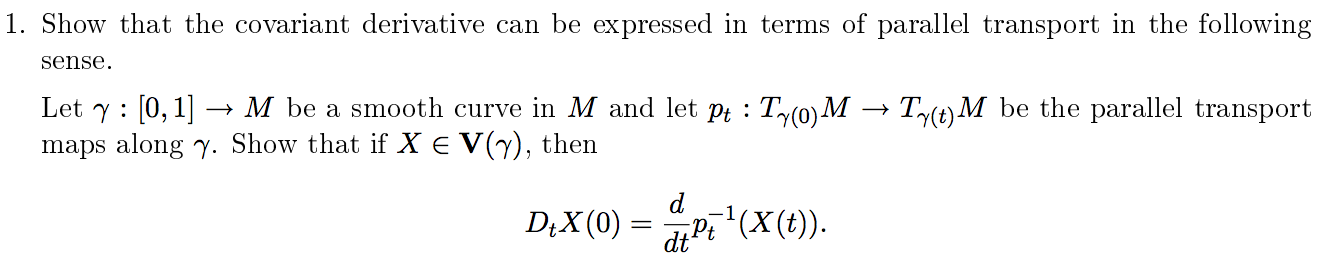
\includegraphics[width=0.7\textwidth]{geo2-s1-p1.png}
\end{figure}
\end{question}
\begin{solution} \hfill \\
Let $E_1(t), ...., E_n(t)$ be a parallel frame along $\gamma$, and $X \in \mathscr{V}
(\gamma)$. Then,
\eQnb
D_tX(0) &=& \sum_{i} D_t(X^i(0)E_i(0)) = \sum_{i} \dot{X}^{i}(0)E_i(0) + 
\sum_{i} X^{i}(0)D_t(E_i(0)) \label{eq:1-1-1} \\
&=& \sum_{i} \dot{X}^{i}(0)E_i(0) 
= \dfrac{d}{dt} \sum_{i} X^{i}(0) P_t^{-1}(E_i(0)) = \dfrac{d}{dt} P_t^{-1}(X(0)) 
\label{eq:1-1-2} \\
&=& \dfrac{d}{dt}|_{t=0}  P_t^{-1}(X(t)) \nonumber 
\eQne
where~\eqref{eq:1-1-1} follows from the Leibiniz rule with $D_t(E_i(0)) = 0$ for
all $i$, and~\eqref{eq:1-1-2} holds by
the linear isomorphism property of $P_t$. \hfill $\qed$ 

\end{solution}


\newpage

\begin{question}[1-2]
\hfill
\begin{figure}[h!]
  \centering
    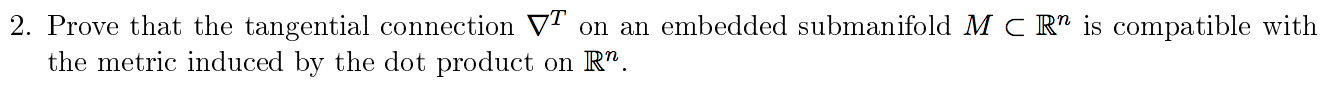
\includegraphics[width=0.7\textwidth]{geo2-s1-p2.png}
\end{figure}
\end{question}
\begin{solution} \hfill \\
Let $\gamma(t)$ be a curve and $Y,Z \in \mathscr{V}(\gamma)$. Then,
\eQnb
\partial_t<Y,Z> &=& <\overline{\triangledown}_{\gamma(t)}Y,Z> + <Y, \overline{
\triangledown}_{\gamma(t)}Z> \nonumber \\
&=& <\pi^{T}(\overline{\triangledown}_{\gamma(t)}Y), Z> + 
<Y,\pi^{T}(\overline{\triangledown}_{\gamma(t)}Z)> \label{eq:1-2-1} \\ 
&=& <\triangledown^{T}_{\gamma(t)} Y, Z> + <Y, \triangledown^{T}_{\gamma(t)}Z> 
\label{eq:1-2-2} 
\eQne
where~\eqref{eq:1-2-1} holds as $Y,Z \in \mathscr{V}(\gamma)$, and~\eqref{eq:1-2-2}
follows from definition of tangential connection. 
Therefore, we have precisely shown the compatibility of the tangential connection
with the metric induced by the dot product on $\mathbb{R}^n$. \hfill $\qed$ 
\end{solution}

\newpage

\begin{question}[1-3]
\hfill
\begin{figure}[h!]
  \centering
    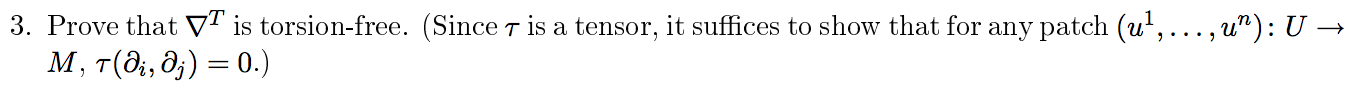
\includegraphics[width=0.7\textwidth]{geo2-s1-p3.png}
\end{figure}
\end{question}
\begin{solution} \hfill \\
Let $X,Y \in \mathscr{V}(M)$. Then,
\eQnb
\triangledown_{X}^{T} Y - \triangledown_{Y}^{T} X &=& 
\pi^{T}(\overline{\triangledown}_{X} Y) - \pi^{T}(\overline{\triangledown}_{Y} X) 
= \pi^{T}(\overline{\triangledown}_{X} Y - \overline{\triangledown}_{Y} X) \nonumber \\ 
&=& \pi^{T}([X,Y]) \label{eq:1-3-1} \\
&=& [X,Y] \label{eq:1-3-2} 
\eQne
where~\eqref{eq:1-3-1} follows from the fact that $\overline{\triangledown}$ is
torsion-free, and~\eqref{eq:1-3-2} follows from $[X,Y] \in \mathscr{V}(M)$. \hfill
$\qed$

\end{solution}

\newpage

\begin{question}[1-4]
\hfill
\begin{figure}[h!]
  \centering
    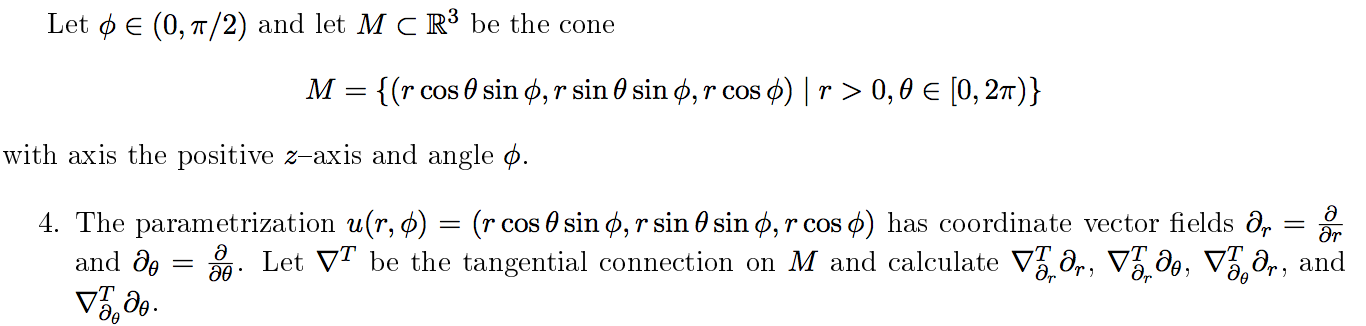
\includegraphics[width=0.7\textwidth]{geo2-s1-p4.png}
\end{figure}
\end{question}
\begin{solution} \hfill \\
We compute
\eQb
\partial_r &=& 
(\cos(\theta)\sin(\phi), \sin(\theta)\sin(\phi), \cos(\phi))\\
\partial_{\theta} &=& 
(-r \sin(\theta) \sin(\phi), r\cos(\theta)\sin(\phi), 0)
\eQe
and hence
\eQb
\overline{\triangledown}_{\partial r} \partial r &=& \dfrac{\partial}{\partial_r}(
\cos(\theta)\sin(\phi), \sin(\theta)\sin(\phi), \cos(\phi)) = (0,0,0) \\ 
\overline{\triangledown}_{\partial r} \partial \theta &=&
\dfrac{\partial}{\partial_r}
(-r \sin(\theta) \sin(\phi), r\cos(\theta)\sin(\phi), 0) 
\\ &=& (-\sin(\theta)\sin(\phi), \cos(\theta)\sin(\phi),0) \\
\overline{\triangledown}_{\partial \theta} \partial r &=&
\dfrac{\partial}{\partial_r}
(\cos(\theta)\sin(\phi), \sin(\theta)\sin(\phi), \cos(\phi))\\
&=& (-\sin(\theta)\sin(\phi), \cos(\theta)\sin(\phi),0) \\
\overline{\triangledown}_{\partial \theta} \partial \theta &=&
\dfrac{\partial}{\partial_r}
(-r \sin(\theta) \sin(\phi), r\cos(\theta)\sin(\phi), 0) \\ 
&=& (-r\cos(\theta)\sin(\phi), -r\sin(\theta)\sin(\phi), 0)
\eQe
Now, to carry out the projection onto the tangent plane, we must obtain the normal.
We compute
\eQb
\partial_r \times \partial_{\theta} &=& (-r\cos(\theta)\sin(\phi)\cos(\phi), 
-r\sin(\theta)\sin(\phi)\cos(\phi), r\sin^2(\phi)) \\ 
\eQe
and hence
\eQb
N &=& \dfrac{\partial_r \times \partial_{\theta}}{|| \partial_r \times \partial_{
\theta} ||} = (-\cos(\theta)\cos(\phi), -\sin(\theta)\cos(\phi), \sin(\phi)). \\ 
\eQe
Therefore, 
\eQb
\triangledown_{\partial_r}^{T} \partial_r &=& (0,0,0) \\
\triangledown_{\partial_{\theta}}^{T} \partial_r &=& 
\triangledown_{\partial_{r}}^{T} \partial_{\theta} = 
\pi^{T}(\overline{\triangledown}_{\partial 
\theta} \partial_r) = \pi^{T}(\dfrac{1}{r} \partial_{\theta}) = \dfrac{1}{r}  
\partial_{\theta} \\
\triangledown_{\partial_{\theta}}^{T}(\partial_{\theta}) &=& \pi^{T}(
\overline{\triangledown}_{\partial \theta} \partial_{\theta}) =
\pi^{T}(\cos(\phi)\sin(\phi)r N - r\sin(\phi)^2 \partial_r) = - r\sin(\phi)^2 
\partial_r 
\eQe
as required. 

\bigskip

Later, I realized that this mess maybe be simplified by noting that the non vanishing
Chirstoffel symbols are
\eQb
\Gamma_{\theta r}^{\theta} &=& \Gamma_{r\theta}^{\theta} = \dfrac{1}{r}  \\
\Gamma_{\theta \theta}^{r} &=& - r\sin(\phi)^2
\eQe
so by the Christofeel formula, we can verify the above results as well.

\hfill $\qed$

\end{solution}

\newpage

\begin{question}[1-5]
\hfill
\begin{figure}[h!]
  \centering
    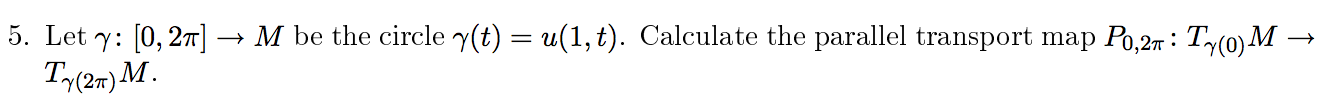
\includegraphics[width=0.7\textwidth]{geo2-s1-p5.png}
\end{figure}
\end{question}
\begin{solution} \hfill \\
Let $\gamma(t) = u(1,t) = (\cos(t)\sin(\phi), \sin(t)\sin(\phi), \cos(\phi))$,
and $V_0 = (V^{r}_0, V^{\theta}_0) \in T_{\gamma(0)}M$. From the transport
equation is given by $D_tV = 0$, and the computations from $1-4$, 
\eQb
D_tV = \dfrac{dV^r}{dt} \partial_r + \dfrac{dV^{\theta}}{dt} \partial_{\theta} 
+ V^r \partial_{\theta} - V^{\theta} \sin(\phi)^2 \partial_r = 0. 
\eQe 
Therefore, $V$ must satisfy the following system of odes: $\dfrac{dV^r}{dt} 
= v^{\theta}\sin(\phi)^2$, $\dfrac{dV^{\theta}}{dt} = -V^r$, with initival conditions
being $V(0) = V_0$. With separation of variables, we see that
\eQb
V^r(t) &=& V_0^r \cos(t\sin(\phi)) + V_0^{\theta} \sin(\phi) \sin(t\sin(\phi)) \\
V^{\theta}(t) &=& V^{\theta}_0 \cos(t \sin(\phi)) - \dfrac{V_0^r}{\sin(\phi)} 
\sin(t\sin(\phi)) 
\eQe  
uniquely solves the system. Therefore, we see that we can give an explicit 
charaterization of the transport map as
\eQb
P_{0,2\pi}(V_0) &=& (\cos(2\pi \sin(\phi)) , \sin(\phi)\sin(2\pi \sin(\phi)) ;
-\dfrac{\sin(2\pi \sin(\phi))}{\sin(\phi)} , \cos(2\pi \sin(\phi))) (V_0^r, 
V_0^{\theta})^{T}
\eQe
for each $V_0 \in T_{\gamma(0)}M$, 
as required. \hfill $\qed$

\end{solution}

\end{document}

